
\chapter{Mathematical Definitions}

In this section we will develop a mathematical perspective of our problem
such that we can focus clearly on the computational aspects in the following
sections. To begin, we are interested in parameterizing polyhedra so we will
develop rigorous definitions of a polyhedra.

The expression of solid bodies is fundamental in the development of any
natural problem statement. For example, in diffusion we model the transfer of
energy throughout a domain. An engineer might define such a domain with a
model, say of an injection molding nozzle. Such a domain is difficult to
describe in terms of a functional boundary, so the engineer might prefer
a boundary representation. Such boundary representations can be converted
to something more natural for numerical methods with software.

In addition to being fundamental to natural studies, solid modeling is growing
in popularity due to low-cost digital manufacturing tools reaching the market.
There have been 3D printers popping up in nearly every educational
institutions over the past 3 years. In addition CNC routing, and laser cutting
enable people to go quickly from design to fabrication.

The development of modern
computational tools for solid modeling have vastly different paradigms. In
the next few sections we will layout the mathematical and computational
principles of these paradigms.

\section{Polyhedra}

Before we define a polyhedra, we must introduce a few notions. These are
solids and orientation. Solids have been studied since
antiquity and for our purposes we will define them as constructions in
three dimensional space with finite volume.
For example, a plane which partitions space is not a solid
since either partition is unbounded, however the intersection of planes
could form a solid.

Orientation is a parallel concept which allows us to specify how geometric
objects contain space. As an example, let us go back to our partition of
space with a plane. If we are on our way to construct a solid, it is
neccessary to choose the one part to keep and the other to discard. This is
the purpose of orientation. In the case of the plane, this follows from the
definition, $ax+by+cz+d=0$. More lucidly, lets look at the signed distance
of a point from the plane, computed as:
\begin{equation}
D = \frac{ax+by+cz+d}{\sqrt{a^2+b^2+c^2}}
\end{equation}
For simplicity, let's look at a plane parallel to the X and Y axes passing
through z = 1. Thus $a$ and $b$ are set to 0, $c$ set to 1, and
$d=-1$
Simplifying our formulation we have:
\begin{equation}
$$ D = 0x+0y+z-1 = z-1$$
\end{equation}
At $z=1$ we see we are on the plane, however at $z=0$ and $z=2$ we get -1 and 1
respectively. The sign of the distance is our indicator of orientation. We can
choose an arbitrary convention as to which partition we will count, but akin
to the "right hand rule" in physics, the normals of the partition must point
outwards. In the case of the plane the normal is the vector $(a,b,c)$, which
in our realization is the upwards vector $(0,0,1)$. Since the convention is
such that the normals point outward, the partition we would consider in a
solid is all points \emph{in the opposite direction of the normal}.
Also to note is the importance of sign in our distance function. We can exploit
this behavior to indicate containment when performing logical operations on
spatial partitions.

Finally we can define a polyhedra in a way useful to us.


\subsection{Implicit Functional Representation}

Implicit functional representation (FRep) in computation centers around a signed, real-value
function where the boundary is defined as $f(...) = 0$.
In $\mathbb{R}3$ this looks like $f(x,y,z) = 0$. For modeling purposes we must add the
additional constraint that the function evaluates to a negative inside the
boundary. Further more the magnitude of the return value must correspond to
the minimum distance between the point and the boundary.\cite{Olah_2011}
A sketch of this behavior in one dimension
can be seen in Figure \ref{fig:implicit-sketch}.

\begin{figure}[h!]
  \centering
    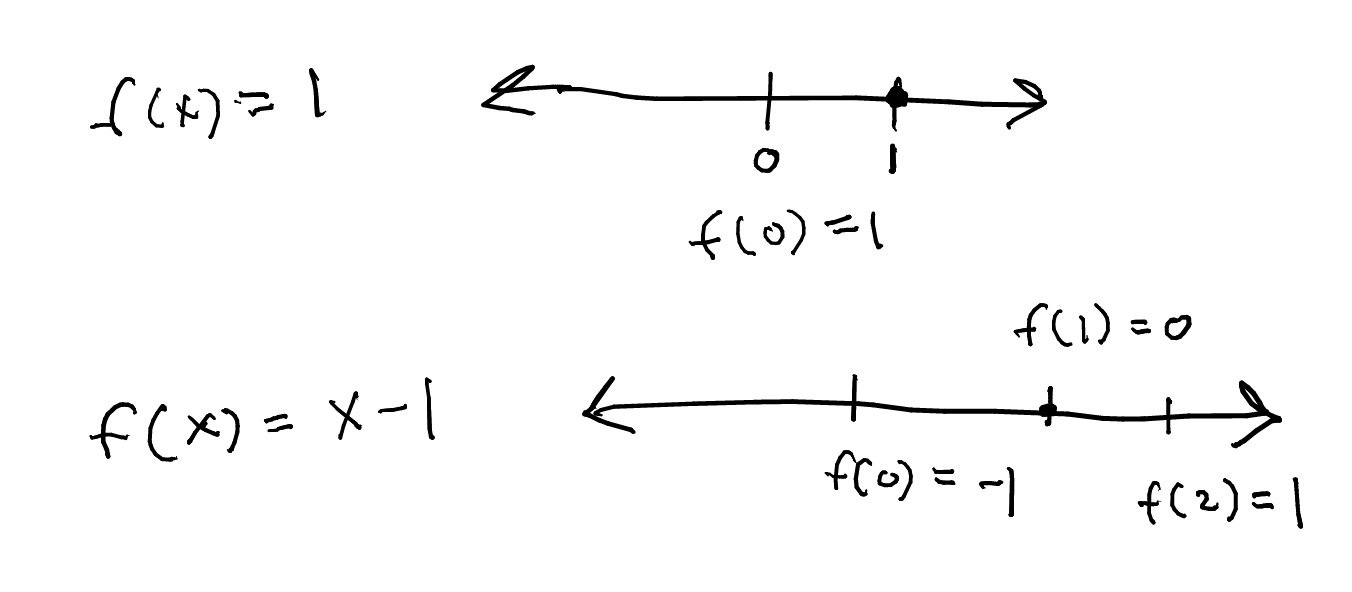
\includegraphics[width=0.75\textwidth]{img/implicit_sketch.png}
  \caption{Number line illustrating the construction of an implicit signed function}
  \label{fig:implicit-sketch}
\end{figure}

Researchers at MIT have taken these principles to constrain
geometric features to ensure a part can be manufactured.\cite{Shugrina_Shamir_Matusik_2015}
They call their system ``FabForms" and shows how functional representations
can easily accept constraints.

One can also compose functional representations with set operations. 
Below are basic set operations defined for these functions:

\begin{equation*}
\cap : \mathtt{min}(f_1,f_2) \\
\end{equation*}
\begin{equation*}
\cup : \mathtt{max}(f_1,f_2) \\
\end{equation*}
\begin{equation*}
\neg : -\mathtt{f}_1
\end{equation*}

It follows that the ``difference"
of $f_1$ and $f_2$ is the intersection of $f_1$ with the negation of $f_2$,
$\mathtt{max}(f_1,-f_2)$.
The mathematical analyst might have trouble with these formulations because
such operations
create discontinuities. This is one area of exploration that will be discussed
later.

More importantly, functional representations can naturally deal with affine
transforms. \cite{Henderson_2002} Given some transform associated with a
FRep, one simply applies the inverse transform to check membership.


\subsection{Signed Distance Fields}

\todo{rewrite to be salient}

A signed distance field (SDF) is a uniform sampling of an implicit function,
or any oriented geometry. \todo{didn't introduce orientation, winding order, etc...}
Below
we can see this in action over the definition of a circle.

\begin{lstlisting}
julia> f(x,y) = sqrt(x^2+y^2) - 1
f (generic function with 1 method)

julia> v = Array{Float64,2}(5,5) # construct a 2D 5x5 array of Float64

julia> for x = 0:4, y = 0:4
           v[x+1,y+1] = f(x,y)
       end

julia> v
5x5 Array{Float64,2}:
 -1.0  0.0       1.0      2.0      3.0    
  0.0  0.414214  1.23607  2.16228  3.12311
  1.0  1.23607   1.82843  2.60555  3.47214
  2.0  2.16228   2.60555  3.24264  4.0    
  3.0  3.12311   3.47214  4.0      4.65685
\end{lstlisting}

The results of \texttt{v} might be confusing since the matrix is oriented with
the origin in the top left corner. At coordinate $(0,0)$, or entry \texttt{v[1,1]},
we see that \texttt{f} is
equal to \texttt{-1}. Likewise we can see $(0,1)$ and $(1,0)$ are points on
the boundary since the value is \texttt{0} and everywhere else is positive.

Distance fields are interesting since they provide an intermediate representation
between functional space and discrete-geometric space. However they are
a very memory hungry data structure. Pixar has published OpenVDB which helps
work around these concerns, but such compression can be lossy.\cite{OpenVDB}
With the advent of shader pipelines for GPUs, distance fields have become
more popular. Valve has used SDFs with great success for generating smooth
text.text renders. \cite{Green_2007}
Many algorithms for generating polyhedra from an SDF
exist. The most common are Marching Tetrahedra, Marching Cubes,
and Dual Contours.\cite{Muller_Wehle_1997}\cite{Newman_Yi_2006}\cite{Cook_Hourvitz}

\todo{Talk about vert and frag shaders.}

Andreas Bærentzen and Henrik Aanæs published methods on the inverse
problem of converting a mesh to a signed distance fields.\cite{Baerentzen_Aanaes}
DiFi was introduced in 2004, which demonstrates an algorithm for creating
SDFs on multiple types of geometry \cite{Sud_Otaduy_Manocha_2004}.
\todo{Need to re-read this paper}

Many necessary algorithms in path planning for digital manufacturing tools
fall out of distance fields. For example, offsetting simply becomes
an addition or subtraction over the SDF. Computing the medial axis becomes
a scan for inflection points. Many path planners need to simplify polygon
representations as to not generate move less than the resolution of the machine.
Assuming the machine uses a Cartesian system, a SDF can correspond perfectly
to the lowest available resolution of the machine.
Likewise as Stereolithographic 3D printers
begin to use digital mirror devices (commonly known as DLP or DMD)
, discrete representations of geometry will become more important in
digital manufacturing.

\subsubsection{Polygonal Meshes}




\subsubsection{Ray Tracing and Marching}

\todo{leave this section, would be good to discuss angle-based polyhedra
and or deficits for these ops}

When we look at the natural world we observe the
propogation of light energy. Our eyes recieve this light energy in the form
of photons. The study of ray tracing seeks to mimic such behavior for
computer visualizations and simulations. 

\begin{figure}[h!]
  \centering
    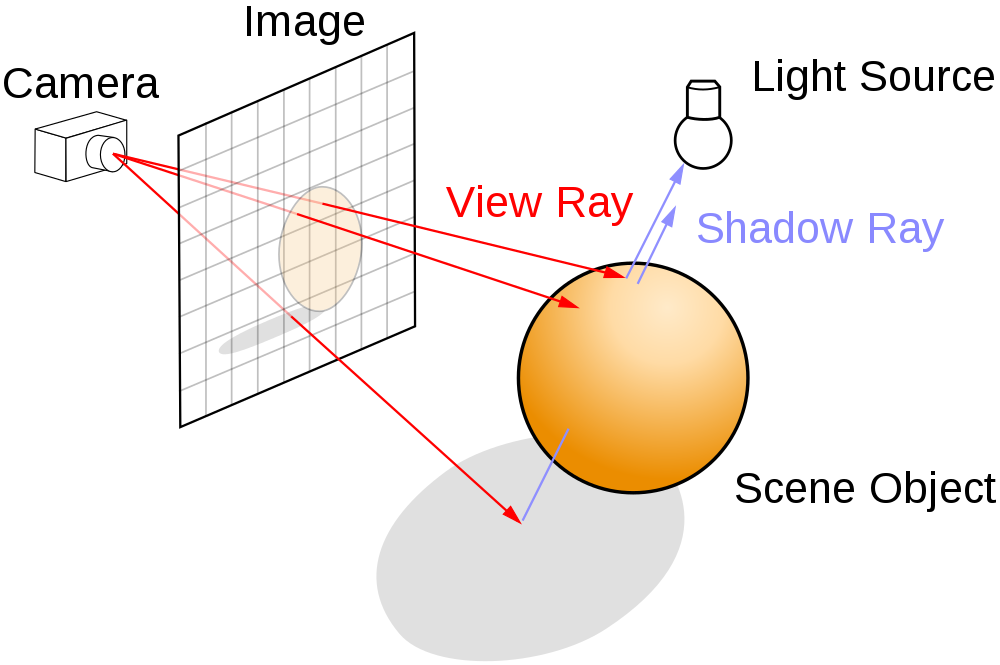
\includegraphics[width=0.75\textwidth]{img/ray_trace_diagram.png}
  \caption{An illustration of a Ray tracing.\protect\footnotemark}
  \label{fig:raytrace}
\end{figure}

\footnotetext{By Henrik (Own work) GFDL or CC BY-SA 4.0-3.0-2.5-2.0-1.0, via Wikimedia Commons}

Íñgo Quílez has done some of the most accessible work on real-time ray tracing.
His technique is called ray marching, and leverages the properties of functional
geometry.\cite{Quilez_2008}

\section{Exploration}

\cite{Pasko_Adzhiev_Comninos_2008}

\subsubsection{Numerical Robustness}

Numerical robustness is a perennial problem in computational geometry. Multiple
approaches exists for various numeric types. Floating points are by far
the most difficult to deal with. Tools such as Gappa have been developed so
algorithm writers can check their invariants when using floating points. \cite{Gappa}
Such tools complicate software development and are not an accessible option
for the casual researcher.

One of the most common problems formulated is to determine whether or not a
point is collinear with a line segment. Shewchuk has one of the most pragmatic
and robust treatments on this topic.\cite{Shewchuk} Kettner, et. al. have also
developed more examples where numerical robustness is critical. \cite{Kettner_Mehlhorn_Pion_Schirra_Yap_2008}

Julia's GeometricalPredicates package \footnote{\url{https://github.com/JuliaGeometry/GeometricalPredicates.jl}}
uses the approach outlined by Volker Springel, which requires all floating point
numbers to be scales between 1 and 2.\cite{Springel_2010} This has the downside
of significantly reducing the available resolution. \todo{why}

A simpler, although less applicable, approach is to work
within integer space. Developing a system around this is of interest. For
example, it should be possible to specify a minimum unit (e.g. microns)
and perform all computations in integer space assuming this does not exceed
the needed resolution. More importantly, modern CPUs have integrated 128 bit
Integer support. 170141183460469231731687303715884105727 is a lot of microns.

\subsubsection{Simplices}

Recently a Simplex type was added to GeometryTypes. A Simplex is defined
as the minimum convex set containing the specified points. The initial
prototype is very simple yet works well. Below we can see a 0th and 1st order
simplex constructed in $\mathbb{R}2$ and $\mathbb{R}3$
\begin{lstlisting}
julia> using GeometryTypes

julia> Simplex(Point(1,2))
GeometryTypes.Simplex{1,FixedSizeArrays.Point{2,Int64}}((FixedSizeArrays.Point{2,Int64}((1,2)),))

julia> Simplex(Point(1,2,3), Point(4,5,6))
GeometryTypes.Simplex{2,FixedSizeArrays.Point{3,Int64}}((FixedSizeArrays.Point{3,Int64}((1,2,3)),FixedSizeArrays.Point{3,Int64}((4,5,6))))
\end{lstlisting}

This representation makes it possible to write code based on the order and
dimensionality of a simplex. Few algorithms have been developed around the
new Simplex type, and unfortunately it is not integrated as a lower-level
construct for the other types yet.

In addition I would like to add a Simplical Complex type.\footnote{\url{https://en.wikipedia.org/wiki/Simplicial_complex}}

\subsubsection{Mesh Slicing}

Topology. Paper by Emmanuel would be a good start.

\subsection{Automatic Differentiation}

\subsubsection{Dual Numbers}
\begin{lstlisting}
julia> using DualNumbers

julia> f(x) = 2x+1
f (generic function with 1 method)

julia> f(Dual(1,1))
3 + 2du
\end{lstlisting}


\subsubsection{Rvachev Functions}


In the 1960's Vladimir Rvachev produced a method for handling the "inverse
problem of analytic geometry". His theory consists of functions which provide a
link between logical and set operations in geometric modeling and analytic
geometry.\cite{shapiro1991theory} I believe the following anecdote helps
elucidate the theory. While attempting to solve boundary value problems,
Rvachev formulated an equation of a square as
\begin{equation*}
a^2 + b^2 − x^2 − y^2 + \sqrt[]{( a^2 − x^2 )^2 +( b^2 − y^2 )^2} =0
\end{equation*}

Implicitly, the sides of a square can be defined as $x= +/- a$ and $y= +/- b$.
The union of these two is a square. By reducing the formulation of the square
we can generalize an expression for the union between two functions.
\begin{equation*}
\cup : f_1 + f_2 + \sqrt[]{f_1^2 +f_2^2} =0
\end{equation*}

Likewise we can see that intersections and negations can be formed for logical
completion.
\begin{equation*}
\cap : f_1 + f_2 - \sqrt[]{f_1^2 +f_2^2} =0 \\
\end{equation*}
\begin{equation*}
\neg : -f_1
\end{equation*}

These formulations can be modified for $C^m$ continuity for any $m$.
\todo{show this construction, it isn't obvious}
\cite{shapiro2007semi} In addition Pasko, et. al. have shown that Rvachev
functions can serve to replace a geometry kernel by creating logical
predicates. \cite{pasko1995function} Their research also establishes the
grounds for user interfaces and environment description. For this work a
practical implementation will most likely leverage their insights.
Rvachev and Shapiro have also shown that using the POLE-PLAST and SAGE
systems a user can generate complex semi-analytic geometry
as well.\cite{rvachev2000completeness} 

While a functional representation for geometry is mathematically enticing on
its own, the power it gives for numerical analysis might be its greatest
virtue. Numerical analysis justified the initial investigation by Rvachev
early on. A boundary value problem on a R-Function-predicate domain allows
for analysis without construction of a discrete mesh.\cite{rvachev2000completeness}

One of the most general expositions in the English language of R-Functions
applied to BVPs is
Vadim Shapiro's``Semi-Analytic Geometry with R-Functions". \cite{shapiro2007semi}
Unfortunately, no monographs about R-Functions exist in the English literature.
Most literature is in Russian, however many articles presenting applied
problems using the R-Function Method. \cite{voron2010}

Such a system for analytic geometry can be developed further. In the context
of an Eulerian flow field, a distance field over a function that
generates partial derivatives could be a fast numerical computation method.

\chapter{Foo}


We began by implementing a Simplex type, defined as follows:

\begin{lstlisting}
"""
A `Simplex` is a generalization of an N-dimensional tetrahedra and can be thought
of as a minimal convex set containing the specified points.

* A 0-simplex is a point.
* A 1-simplex is a line segment.
* A 2-simplex is a triangle.
* A 3-simplex is a tetrahedron.

Note that this datatype is offset by one compared to the traditional
mathematical terminology. So a one-simplex is represented as `Simplex{2,T}`.
This is for a simpler implementation.

It applies to infinite dimensions. The sturucture of this type is designed
to allow embedding in higher-order spaces by parameterizing on `T`.
"""
immutable Simplex{N,T} <: AbstractSimplex{N,T}
    _::NTuple{N,T}
end
\end{lstlisting}

With the definition in GeometryTypes, we afford ourselves two notions of
dimensionality. Our first parameter `N` gives us the total dimensionality
of the simplex. `T` is the type of the points. For example in Julia we can
prefix a colon to an identifier and make it a symbol which is reflected
in the type information:

\begin{lstlisting}
julia> using GeometryTypes

julia> Simplex(:x,:y,:z)
GeometryTypes.Simplex{3,Symbol}((:x,:y,:z))
\end{lstlisting}

Symbolic representation will allow us to create parametric geometry.
Likewise we can construct concrete types:

\begin{lstlisting}
julia> Simplex(Point(0,0,0), Point(1,1,1))
GeometryTypes.Simplex{2,FixedSizeArrays.Point{3,Int64}}((FixedSizeArrays.Point{3,Int64}((0,0,0)),FixedSizeArrays.Point{3,Int64}((1,1,1))))
\end{lstlisting}

This last example illustrates how this type can give us extra generalization.
Here we have constructed a line segment in 3D space. The Simplex is of
size two but the space it occupies is three dimensional. This way it acts
similar to a fixed size vector, but the type implies all points are on the
convex hull. (Should update decription to be accurate here).

Below is an example of a high performance implementation of Simplex decomosition:

\begin{lstlisting}
"""
Decompose an N-Simplex into tuple of Simplex{2}
"""
@generated function decompose{N, T1, T2}(::Type{Simplex{2, T1}},
                                       f::Simplex{N, T2})
    # other wise degenerate
    2 <= N || error("decompose not implented for N <= 2 yet. N: $N")

    v = Expr(:tuple)
    append!(v.args, [:(Simplex{2,$T1}(f[$(i)],
                                        f[$(i+1)])) for i = 1:N-1])
    # connect vertices N and 1
    push!(v.args, :(Simplex{2,$T1}(f[$(N)],
                                     f[$(1)])))
    v
end
\end{lstlisting}




To some extent, much of the basic defintions have been implemented
in libraries such as CGAL, Boost, and ShapeOP. However these libraries
are written in C and C++, compiled langauges, that are not amicable to dynamic
exploration. Our system should allow us to quickly prototype tests and
visualize relationships. This is something that Julia provides extremely well.
Primarily it accomplishes this through optional type annotations and
multiple dispatch. Secondarily, it has a rich history of integration with
interactive computing environments such as a REPL, Jupyter, and Juno.


Prior to this project, GeometryTypes primarily provides for Polygonal Mesh
type that is well tuned for operations on the CPU and GPU. It is defined
as follows:

\begin{lstlisting}
"""
The `HomogenousMesh` type describes a polygonal mesh that is useful for
computation on the CPU or on the GPU.
All vectors must have the same length or must be empty, besides the face vector
Type can be void or a value, this way we can create many combinations from this
one mesh type.
This is not perfect, but helps to reduce a type explosion (imagine defining
every attribute combination as a new type).
"""
immutable HomogenousMesh{VertT, FaceT, NormalT, TexCoordT, ColorT, AttribT, AttribIDT} <: AbstractMesh{VertT, FaceT}
    vertices            ::Vector{VertT}
    faces               ::Vector{FaceT}
    normals             ::Vector{NormalT}
    texturecoordinates  ::Vector{TexCoordT}
    color               ::ColorT
    attributes          ::AttribT
    attribute_id        ::Vector{AttribIDT}
end
\end{lstlisting}

The first thing to note is the provisions for attributes, colors, and textures.
These are used for mapping textures and/or colors to polygons via APIs such as
OpenGL. We do not need these (at least yet) in a rigourous mathematical
definition. Likewise, in a HomogenousMesh we structure the realization as
follows: 1. Insert all vertices of the mesh into `vertices` 2. Construct
Faces of at least 3 indices referencing the points in `vertices`.

This gives us certain properties that are nice for computation. Primarily
this allows us to observe the combinatorial properties of the mesh by analyizing
the faces. In addition, this compacts the data representation of vertices
since shared vertices can be represented with a common face index. Affine
transforms only need to operate on the vertices. Thus, in the optimistic versus
pessimistic case these operations can be 3x faster with this layout
assuming all vertices are in 3 faces.

Maybe a good idea to implement on this type too?

